\chapter{Herramientas}
\label{chap:herramientas}
En este capítulo se van a detallar las herramientas y tecnologías utilizadas en el desarrollo de este proyecto principalmente en el ámbito web. Algunas se han elegido por facilidad de uso y otras por necesidad del entorno desarrollado.

% JAVASCRIPT %
\section{JavaScript}
\label{sec:js}
\textit{JavaScript} es un lenguaje interpretado de alto nivel que se encuentra bajo el estándar \textit{ECMAScript}\footnote{Especificación de lenguaje de programación el cual define tipos dinámicos y soporta características de programación orientada a objetos.} y está basado en otros lenguajes de programación como Java o C. 

En su principio fue concebido como lenguaje de aplicaciones web para el lado cliente, interpretado en un navegador web, permitiendo mejorar la interfaz de usuario y realizar páginas web dinámicas.

En la actualidad, \textit{JavaScript} se ha ido extendiendo hacia el lado servidor con \textit{Node.js} y es por ello que es el lenguaje más utilizado para desarrollo web y todos los navegadores interpretan el código integrado en las páginas web.

Para este proyecto se ha usado \textit{ECMAScript 6} o \textit{ECMAScript 2015} y, como el proyecto se orienta a la creación de una aplicación con todo el peso en el lado del cliente, \textit{JavaScript} es el lenguaje que mejor se adapta a los requerimientos del desarrollo. De esta manera, se ha programado toda la inteligencia de la aplicación web, que corre en el navegador. 

Las siguientes características son las principales de ECMAScript: 
\begin{itemize}
    \item Es un lenguaje estructurado, tiene gran similitud con \textit{C} y comparte gran parte de su estructura (bucles, condicionales, sentencias...) a excepción del alcance de sus variables. En \textit{C} su ámbito es el bloque en el que fue definida y, en su origen, \textit{JavaScript} tenía un alcance global en las variables definidas. Es en ECMAScript 2015 cuando se añade la palabra clave \textit{let}, que incorpora compatibilidad con \textit{block scoping} (alcance de la variable en el bloque en la que es definida). 
    \item Tipado débil, por el cual el tipo de datos está asociado al valor, no a la variable. Esto significa que una variable puede ser \textit{number} o \textit{string} en distintos momentos de ejecución. 
    \item Formado en su totalidad por objetos, en los cuales los nombres de sus propiedades son claves de tipo cadena siendo \textit{objeto.a = 1} y \textit{objeto['a'] = 1} equivalentes. 
    \item Lenguaje interpretado, es por esto que no requiere un compilador ni crear un fichero binario del código; cada navegador tiene su intérprete que se encarga de ejecutarlo.
    \item Evaluación en tiempo de ejecución gracias a la función \textit{eval}, la cual evalúa un código en \textit{JavaScript} representado como una cadena de caracteres. 
\end{itemize}
% A-FRAME %
\section{A-Frame}
\label{sec:aframe}
\textit{A-Frame} es un entorno de código abierto destinado a crear experiencias de realidad virtual a partir de \textit{HTML} de forma que sea sencillo de leer y comprender. De esta manera es accesible para crear una gran comunidad. \textit{A-Frame} está en constante desarrollo, pero la versión utilizada en este proyecto es la última versión estable (\textit{v0.9.2}) y se ha utilizado este framework por la facilidad de crear escenarios tridimensionales a través de un documento \textit{HTML} y de añadir modelos sofisticados en distintos formatos.

Además tiene compatibilidad con \textit{Vive}, \textit{Rift}, \textit{Windows Mixed Reality}, \textit{Daydream}, \textit{GearVR} y \textit{CardBoard} así como soporte para todos los controladores respectivos. También ofrece soporte para ordenadores de escritorio y para la mayoría de teléfonos inteligentes.

\subsection{HTML y primitivas}
\textit{A-Frame }se basa en \textit{HTML} y el \textit{DOM} usando un \textit{polyfill}\footnote{Fragmento de código en \textit{JavaScript} utilizado para proporcionar una funcionalidad moderna en navegadores antiguos.} para elementos personalizados. \textit{HTML} es un componente básico para Web y como tal, tiene una gran accesibilidad como lenguaje. Para crear una escena de realidad virtual con \textit{A-Frame} no se requiere ninguna instalación y simplemente con la creación del \textit{HTML} se puede abrir en el navegador. La mayoría de herramientas existentes (como \textit{React}, \textit{Vue.js}, \textit{d3.js} y \textit{jQuery}) funcionan en este entorno. 

\textit{HTML} y \textit{DOM} son solo la capa más externa del framework, debajo se encuentra el componente \textit{three.js} en el que está basado \textit{A-Frame} gracias al cual un componente puede ser utilizado en distintas entidades. De esta manera hace posible seguir el principio de programación \textit{Don't Repeat Yourself} ya que, una vez registrada una primitiva, se puede hacer referencia al elemento todas las veces que sea necesario.  

A-Frame proporciona elementos como \textit{a-box} o \textit{a-sky} llamados primitivas. Podemos crear un escenario a través de estas primitivas como el mostrado en la figura \ref{fig:scene1} con el siguiente código: 

\begin{lstlisting}[language=javascript, caption=Código con primitivas que representa un escenario]
<!DOCTYPE html>
<html>
  <head>
    <meta charset="utf-8">
    <title>Escenario primitivas</title>
    <script src="https://aframe.io/releases/0.9.2/aframe.min.js"></script>
  </head>
  <body>
    <a-scene background="color: #FAFAFA">
      <a-box position="-1 0.5 -3" rotation="0 45 0" color="#4CC3D9" shadow></a-box>
      <a-sphere position="0 1.25 -5" radius="1.25" color="#ff0000" shadow></a-sphere>
      <a-cylinder position="1 0.75 -3" radius="0.5" height="1.5" color="#FFC65D" shadow></a-cylinder>
      <a-plane position="0 0 -4" rotation="-90 0 0" width="4" height="4" color=" #1cde83" shadow></a-plane>
      <a-sky color="#e7e1e0"></a-sky>
    </a-scene>
  </body>
</html>
\end{lstlisting}

\begin{figure}[H]
\centering
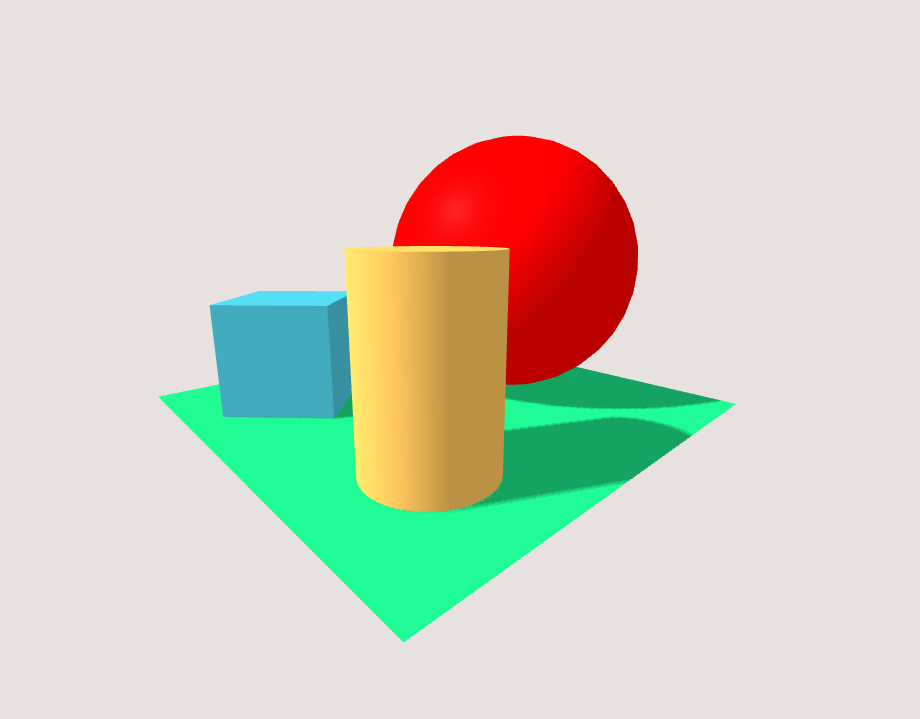
\includegraphics[width=0.8\textwidth]{img/scene1.png}
\caption{Escenario a-frame} \label{fig:scene1}
\end{figure}

A-Frame, además de disponer primitivas como las mostradas, hace posible la creación de primitivas para poder elaborar escenas lo más completas posible. También se pueden incluir entidades más complejas a partir de modelos 3D en formatos como \textit{gltf}, \textit{obj} o \textit{collada} de los cuales se hablará en siguientes apartados.

\subsection{Entidad, Componente y Sistema}

    Como ya se ha comentado, A-Frame es un entorno \textit{three.js} con una arquitectura de entidad-componente-sistema (\textit{ECS}). Es un patrón común en 3D y desarrollo de juegos que siguen la composición sobre el principio de herencia y jerarquía. Algunos beneficios que \textit{ECS} aporta son mayor flexibilidad al definir objetos, gran escalabilidad o eliminación de problemas de largas cadenas de herencia. Existe un \textit{API} que representa cada pieza de \textit{ECS}: 
    \begin{itemize}
    \item Una entidad se representa con la etiqueta \textit{a-entity}. 
        \begin{lstlisting}[language=HTML]
        <a-entity geometry="primitive: box" material="color: red">
        \end{lstlisting}
        En este ejemplo se hace uso de \textit{a-entity} para crear una caja de color rojo. 

    
    \item Un componente se representa como un atributo de HTML. Cada componente es un objeto que tiene un esquema, manejadores y métodos. Para registrar componentes se utiliza el método de A-Frame \textit{registerComponent}.
    
    \begin{lstlisting}[language=javascript, caption=Código para registrar un componente]
        AFRAME.registerComponent('example', {
          init: function () {
            var el = this.el;
            el.setObject3D('mesh', new THREE.Mesh());
            el.getObject3D('mesh');  // Returns THREE.Mesh that was just created.
          }
        });
    \end{lstlisting}
    
    \item Un sistema es el representado por atributos HTML mediante la etiqueta \textit{a-scene}. Se registran de manera similar a un componente; gracias al método \textit{registerSystem}.
\end{itemize}


% BLOCKLY %
\section{Blockly}
\label{sec:blockly}
\textit{Blockly} es una librería que añade un editor de código visual a aplicaciones web y móviles. Utiliza bloques gráficos para representar conceptos complejos de código de manera más sencilla. De esta manera permite a los usuarios aplicar  principios de programación sin tener que preocuparse por la sintaxis y ayuda a iniciarse y a aprender a programar a estudiantes de temprana edad. Esta librería es un proyecto de \textit{Google} y está diseñada por las personas que están detrás de \textit{Scratch} del \textit{MIT} y construido sobre su base de código. Actualmente se encuentra en su versión \textit{1.20190215} y se ha utilizado para crear bloques que den funcionalidad a los robots empleados en la plataforma. 

\subsection{Traductor de código}
\textit{Blockly} es para desarrolladores y las \textit{aplicaciones Blockly} son pensadas para estudiantes. Desde la perspectiva de usuario, \textit{Blockly} es una forma visual e intuitiva de crear código y, desde la de desarrollador, es una interfaz de usuario preparada para crear un lenguaje visual que emite código y se puede exportar a otros lenguajes de programación como \textit{JavaScript}, \textit{Python}, \textit{PHP}, \textit{Lua} o \textit{Dart}. 

Estos generadores de código aportan las herramientas para crear funciones, condicionales, bucles, etc. El principal problema de esto es que en ocasiones se requiere del uso de APIs de otras dependencias. \textit{Blockly} aporta una solución; un generador de bloques personalizados que traduce al código que deseemos. Esto aporta mucha flexibilidad y da la funcionalidad deseada para el desarrollo de este proyecto. 

\subsection{Bloques personalizados}
Como se ha explicado, \textit{Blockly} dispone de una gran cantidad de bloques predefinidos; desde funciones matemáticas hasta estructuras en bucle. Sin embargo, para interactuar con una aplicación externa, se deben crear bloques personalizados para formar una API. Según la documentación ofrecida por \textit{Google}\footnote{\url{https://developers.google.com/blockly/guides/create-custom-blocks/overview}}, la mejor forma de crear un bloque es buscar un bloque existente con una funcionalidad similar y modificarlo según se necesite. De otra manera, para generar un bloque personalizado, hay varios aspectos a tener en cuenta: 

\begin{itemize}
    \item Primero se define el bloque para determinar su aspecto gráfico y su comportamiento. Esto incluye el texto, color, forma o cómo conectarlos con otros bloques. La configuración de estos parámetros se puede realizar mediante \textit{JSON} o \textit{JavaScript}. El bloque mostrado en la figura \ref{fig:customblock} se puede configurar con los dos métodos de la siguiente manera:
    
     \begin{lstlisting}[language=json, caption=Código en JSON para configurar un bloque personalizado]
     {
      "type": "block_test",
      "message0": "%1 %2",
      "args0": [
        {
          "type": "field_label_serializable",
          "name": "NAME",
          "text": "custom_block"
        },
        {
          "type": "input_value",
          "name": "NAME",
          "check": "Number"
        }
      ],
      "inputsInline": false,
      "previousStatement": null,
      "nextStatement": null,
      "colour": 120,
      "tooltip": "This is a custom block",
      "helpUrl": ""
    }
    \end{lstlisting}

    \begin{lstlisting}[language=javascript, caption=Código en \textit{JavaScript} para configurar un bloque personalizado]
    Blockly.Blocks['block_test'] = {
      init: function() {
        this.appendValueInput("NAME")
            .setCheck("Number")
            .appendField(new Blockly.FieldLabelSerializable("custom_block"), "NAME");
        this.setInputsInline(false);
        this.setPreviousStatement(true, null);
        this.setNextStatement(true, null);
        this.setColour(120);
     this.setTooltip("This is a custom block");
     this.setHelpUrl("");
      }
    };
    \end{lstlisting}

    \begin{figure}[H]
    \centering
    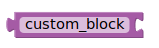
\includegraphics[width=0.2\textwidth]{img/CustomBlock.png}
    \caption{Bloque personalizado} \label{fig:customblock}
    \end{figure}

    \item Configurar la traducción del bloque a la instrucción deseada en los distintos lenguajes necesarios.
    
    \item Inicializar el bloque para que sea visible en el editor visual de código. 
    
    Aunque los parámetros del \textit{JSON} son auto-descriptivos, es complicado generar un bloque desde cero. Es por ello que \textit{Google} facilita  una herramienta de creación de bloques, la cual se muestra en la figura \ref{fig:googleTool}. 
    En ella se puede personalizar todos los aspectos del bloque: texto, color, variables de entrada, formas de conexión con otros bloques, etc.
    Además, da la opción de exportar la configuración del bloque en formato \textit{JSON} o \textit{JavaScript} y muestra una función con la configuración básica para obtener el código en JavaScript (y permite seleccionar el lenguaje deseado entre los admitidos por \textit{Blockly}).
    
    \begin{figure}[H]
    \centering
    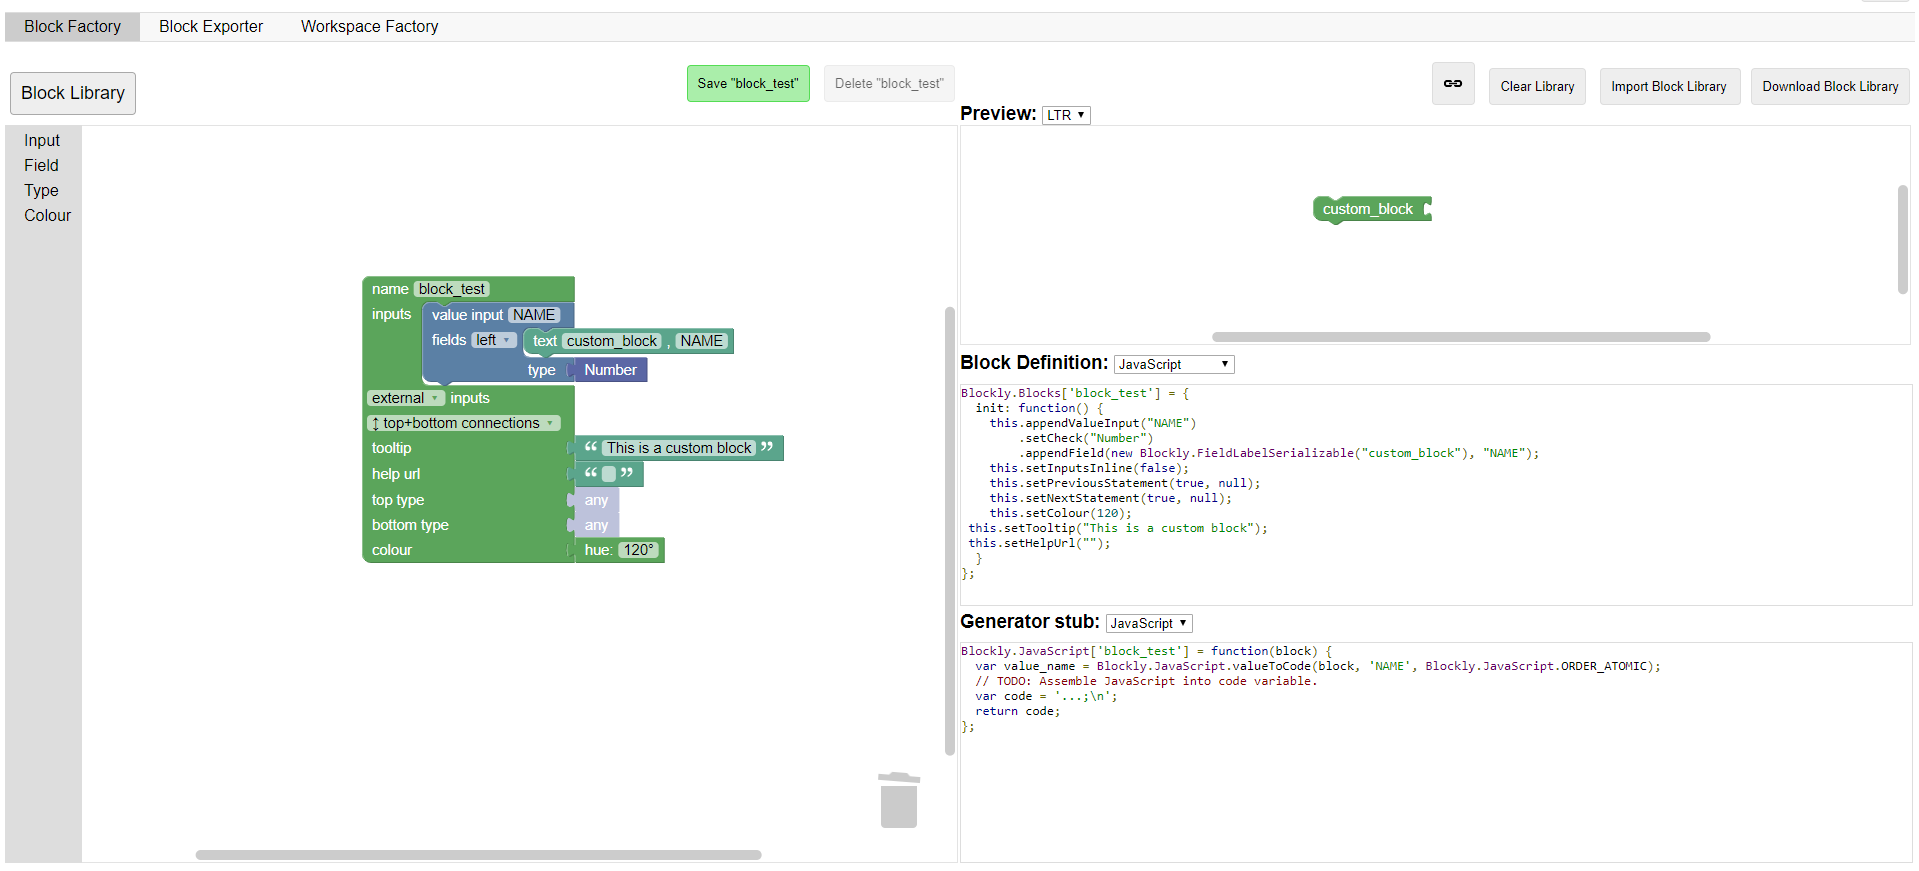
\includegraphics[width=1.1\textwidth]{img/GoogleTool.png}
    \caption{Herramienta para creación de bloques personalizados} \label{fig:googleTool}
    \end{figure}
    
\end{itemize}

% GESTORES DE PAQUETES %
\section{Gestores de paquetes}
\label{sec:gest}
Un gestor de paquetes es una herramienta para automatizar el proceso de instalación, actualización, configuración y eliminación de software. En este proyecto se han utilizado \textit{NPM} y \textit{Webpack} en sus versiones \textit{3.5.2} y \textit{4.41.2} respectivamente. Se han empleado para descargar los paquetes y dependencias para la correcta ejecución de la aplicación y para generar los \textit{bundles} correspondientes. 

\subsection{NPM}
\textit{Node Package Manager}\footnote{\url{https://www.npmjs.com/}} (\textit{NPM}) es el sistema de gestión de dependencias por defecto para \textit{Node.js}, que es un entorno de ejecución para \textit{JavaScript} y permite, con la configuración de un fichero, descargar dependencias y paquetes necesarios para el correcto funcionamiento de la aplicación. Todo ello ha de estar definido en un fichero llamado \textit{package.json} que debe ser escrito en \textit{JSON}. Para usar \textit{NPM} como instalador de paquetes únicamente hay que ejecutar ``\textit{npm install}'' en el directorio en el que se encuentre el fichero \textit{package.json}. Además, gracias a este gestor, podemos configurar pequeños \textit{scripts} para ejecutar algún proceso como lanzar una aplicación después de la instalación o empaquetar la aplicación en \textit{bundles} combinándolo con \textit{Webpack}.

\subsection{Webpack}
\textit{Webpack}\footnote{\url{https://webpack.js.org/}} es un sistema de \textit{bundling} usado para empaquetar una aplicación web en su fase de producción. Se puede considerar una evolución de \textit{Grunt}\footnote{\url{https://gruntjs.com/}} y \textit{Gulp}\footnote{\url{https://gulpjs.com/}} porque permite automatizar procesos principales tales como transpilar y preprocesar código. 


% BLENDER %
\section{Blender}
\label{sec:blender}
\textit{Blender} es un programa libre dedicado al diseño y animación 3D. Mediante una interfaz gráfica permite diseñar objetos, personajes y escenas en tres dimensiones con muy diversas técnicas. Cada uno de los elementos creados pueden ser animados mediante \textit{keyframing} o animación por fotogramas clave. En su origen \textit{Blender} fue distribuido como una herramienta privada explotada por un estudio de animación, pero actualmente se encuentra bajo licencia \textit{GPL}\footnote{\url{https://www.gnu.org/licenses/gpl-3.0.en.html}}. 

La versión utilizada en este proyecto es la \textit{2.79} y se ha empleado para la creación de modelos y escenarios para ser incluidos en el simulador \textit{WebSim}. En la imagen \ref{fig:blender} se puede ver la interfaz gráfica de \textit{Blender}. \\

    
\begin{figure}[H]
    \centering
    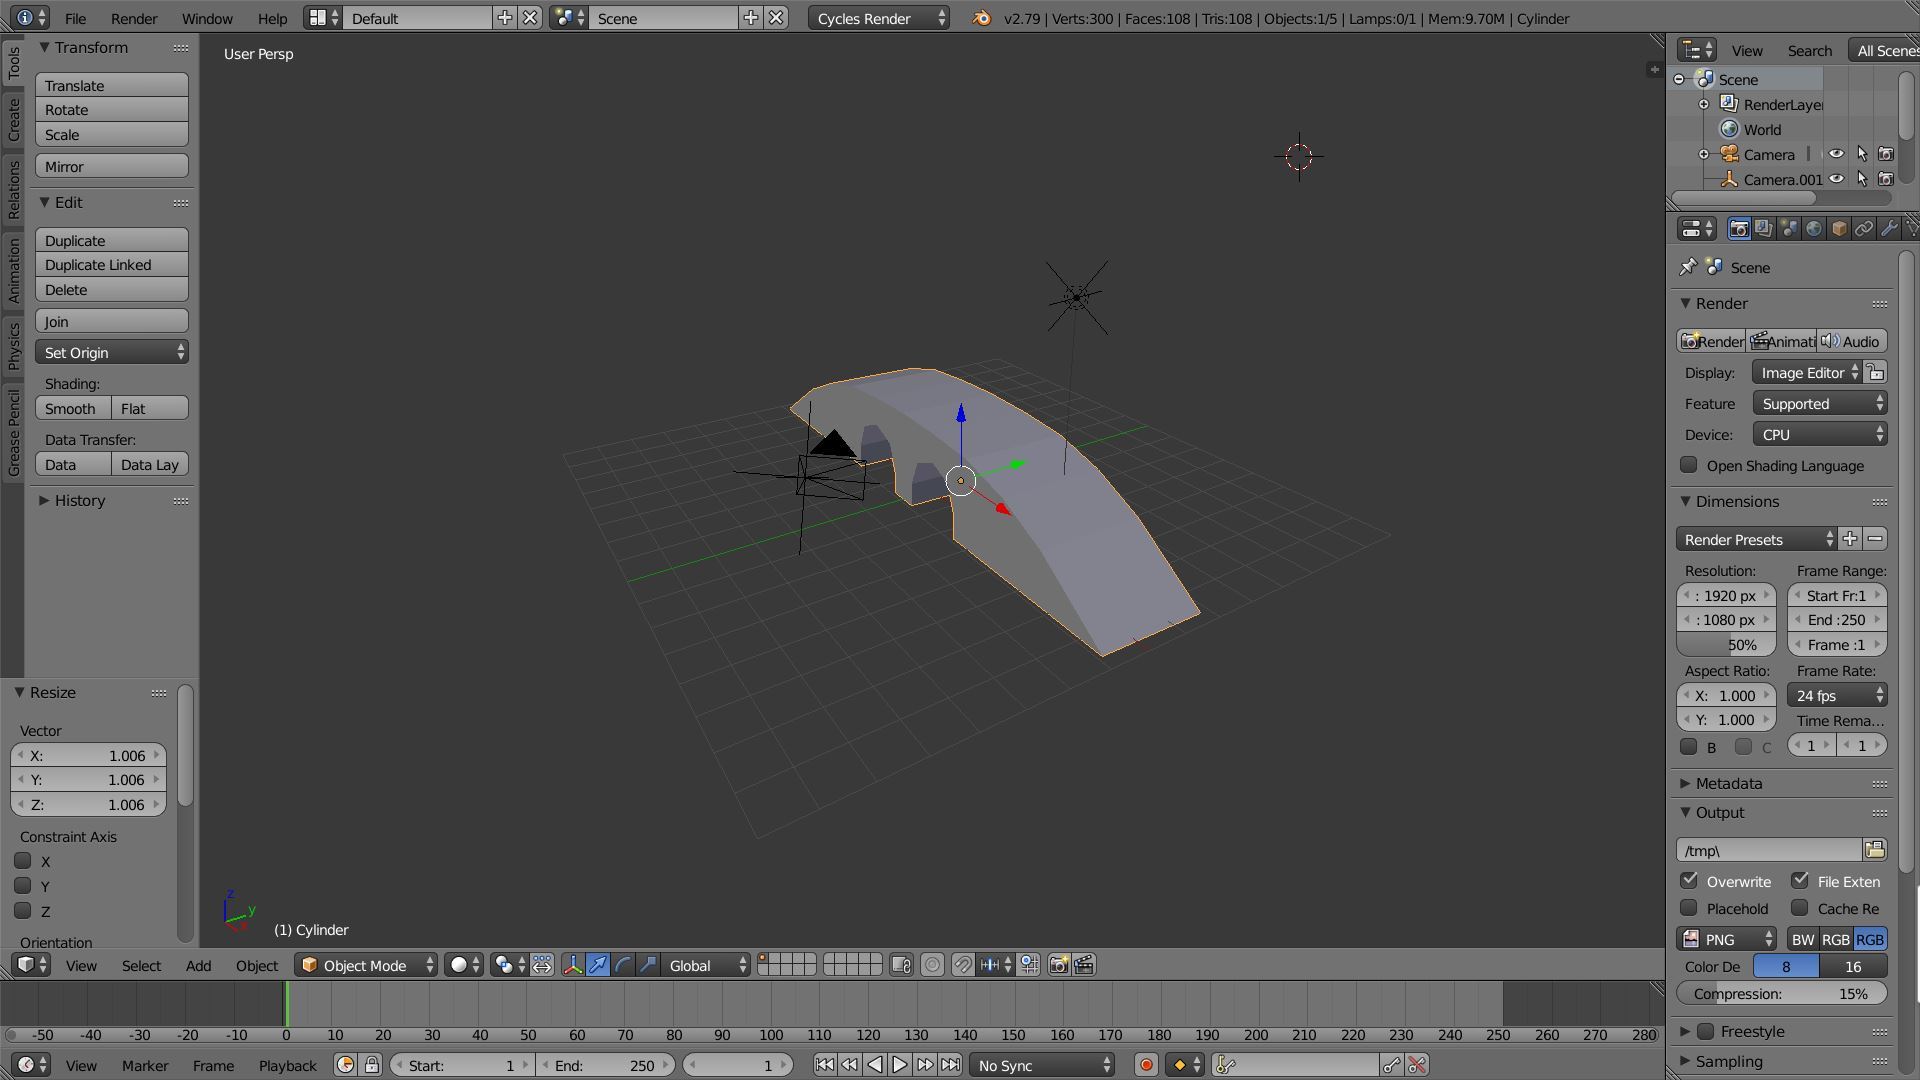
\includegraphics[width=1\textwidth]{img/blender.jpg}
    \caption{Interfaz gráfica de \textit{Blender}} 
    \label{fig:blender}
\end{figure}

Entre las muchas características que ofrece \textit{Blender}, las más útiles para el desarrollo del proyecto son:
\begin{itemize}
    \item \textbf{Modelados}: es el proceso mediante el cual se crean objetos en un espacio 3D de manera digital. Están compuestos de líneas, puntos, cuadrados, triángulos, etc. 
    
    \item \textbf{Iluminación}: existen varios tipos de luz que se pueden adaptar a la escena. Es posible aplicar a cada uno de los objetos para especificar la luz recibida por cada uno de ellos además de variar aspectos como la intensidad, el color o la posición en el escenario.
    
    \item \textbf{Tracking}: permite especificar el comportamiento y características de un determinado objeto en el escenario tridimensional. 
    
    \item \textbf{Animaciones}: cada objeto se puede animar de manera independiente. Se realiza mediante una secuencia de fotogramas en la cual cada instante de tiempo es un fotograma en el cual se especifica cualquier tipo de característica (rotación, movimiento, cambio de color, etc).  
    
    \item \textbf{Texturizado}: son un medio para agregar o eliminar detalles a la superficie de un determinado objeto. Proyectando imágenes sobre la superficie del mallado se pueden aplicar patrones para personalizar el aspecto de la textura. 

    Además permite exportar los modelos a los formatos más usados para \textit{A-Frame}: \textit{glTF} y \textit{COLLADA}. 
\end{itemize}
\subsection{COLLADA}
\textit{COLLaborative Design Activity} (\textit{COLLADA}) es un  formato de archivo de intercambio para aplicaciones 3D interactivas. Se define como un esquema \textit{XML} para intercambiar activos digitales entre varias aplicaciones de software de gráficos. Son definidos con la extensión \textit{.dae} y pueden hacer referencia a archivos de imagen adicionales que actúan como texturas del objeto 3D. 

\subsection{glTF}
GL Transmission Format (\textit{glTF}) es una especificación basada en el estándar \textit{JSON} para transmisión y carga eficiente de escenas y modelos 3D para aplicaciones. Este formato minimiza el tamaño de los ficheros y su tiempo de ejecución necesario para desempaquetar y usarlos. Permite animación de los objetos, que puede ser activada por \textit{A-Frame} vía \textit{HTML} o dinámicamente con \textit{JavaScript}. 
En la imagen \ref{fig:tree} se puede ver la figura añadida a un escenario de A-Frame vía \textit{HTML}:

\begin{lstlisting}[language=html, caption=Código para añadir un modelo 3D personalizado a A-Frame]
 <a-asset-item id="tree" src="assets/models/tree.dae"></a-asset-item>
  <a-entity id="a-tree" collada-model="#tree" rotation="0 0 0" position="2.75 0.01 -2.27">
  
\end{lstlisting}

\begin{figure}[H]
\centering
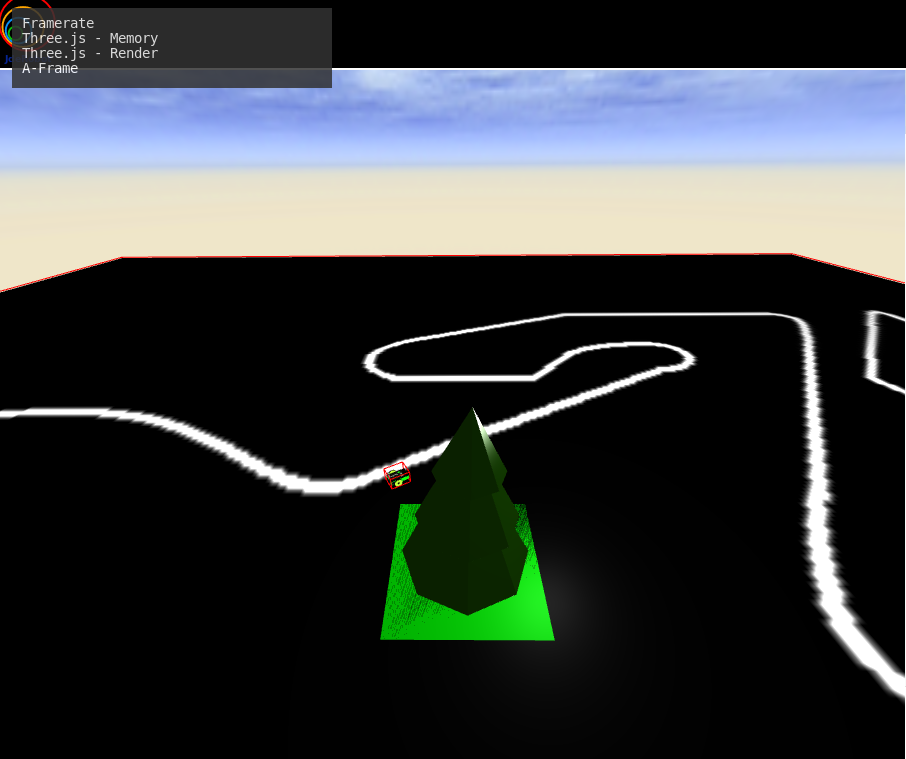
\includegraphics[width=0.8\textwidth]{img/tree_aframe.png}
\caption{Modelo glTF añadido en un escenario de A-Frame} \label{fig:tree}
\end{figure}
Además del \textit{software} explicado en esta sección, existen multitud de herramientas para convertir a glTF desde formatos como \textit{OBJ}, \textit{COLLADA} o  \textit{PCD}\footnote{\url{https://github.com/KhronosGroup/glTF}}. De esta manera es posible buscar modelos 3D en librerías\footnote{\url{https://sketchfab.com}} para editarlos e incluirlos en \textit{Websim}.

% WEBSIM %
\section{Simulador WebSim}

\textit{Websim} es un simulador diseñado para enseñar conceptos básicos de tecnología e iniciar a niños en robótica y programación. La versión inicial de la que parte este proyecto está desarrollada por Álvaro Paniagua Tena\footnote{\url{https://github.com/RoboticsLabURJC/2018-tfg-alvaro_paniagua}} y dada su  importancia en el desarrollo de este TFG, se describe con cierta profundidad.  

\subsection{Diseño}
\label{subsec:design}
El simulador hace uso del entorno \textit{A-Frame} y su diseño permite conectar un editor de texto o un editor de bloques para  programar en \textit{JavaScript} o \textit{Blockly} y conectar este código con el robot simulado. También permite acoplar una aplicación externa al navegador a través de comunicaciones ICE. En la figura \ref{fig:websim} se puede ver el diseño de \textit{WebSim}.

Las principales funcionalidades del simulador son: 

\begin{itemize}
    \item Registrar los componentes principales para constituir un robot en \textit{A-Frame}, los cuales son \textit{followBody},\textit{spectatorComponent} e \textit{intersectionHandler}. El primero se encarga de simular una cámara en el robot, el segundo maneja eventos de intersección de los láseres y el último permite anclar distintos elementos al robot simulado. 
    
    \item Ofrece una interfaz en \textit{JavaScript} para manejar el robot en el entorno simulado de \textit{A-Frame} llamada \textit{Hardware Abstraction Layer} (\textit{HAL API}). \textit{Websim} se encarga de enviar instrucciones al robot de manera sencilla sin necesidad de comunicarse con el motor de \textit{A-Frame}. 
    
    \item No es necesario que el usuario instancie ningún tipo de variable de la clase que contiene al objeto robot porque el simulador lo ofrece de manera directa. De esta manera el usuario puede mandar directamente instrucciones al robot simulado con el objeto \textit{myRobot} y los métodos existentes de la clase \textit{RobotI}.
    
    \item Permite manejar la ejecución de la simulación del robot. Es decir, permite lanzar o pausar la ejecución del robot e incluso reiniciar su posición para no tener que recargar la página en caso de querer probar distintos códigos con la misma simulación. Además este control del entorno evita que la variable \textit{myRobot} pierda el objeto instanciado porque el usuario cambie su valor.
    
\end{itemize}

Gracias a estas características, el simulador hace que los usuarios puedan programar de manera sencilla, ya que solo tienen que acceder a la información que ofrecen los sensores del robot y mandar órdenes sobre los actuadores del mismo. Es decir, solo  se tienen que encargar de programar la lógica del robot para resolver los ejercicios propuestos que se explicarán en próximos capítulos. 


\begin{figure}[H]
    \centering
    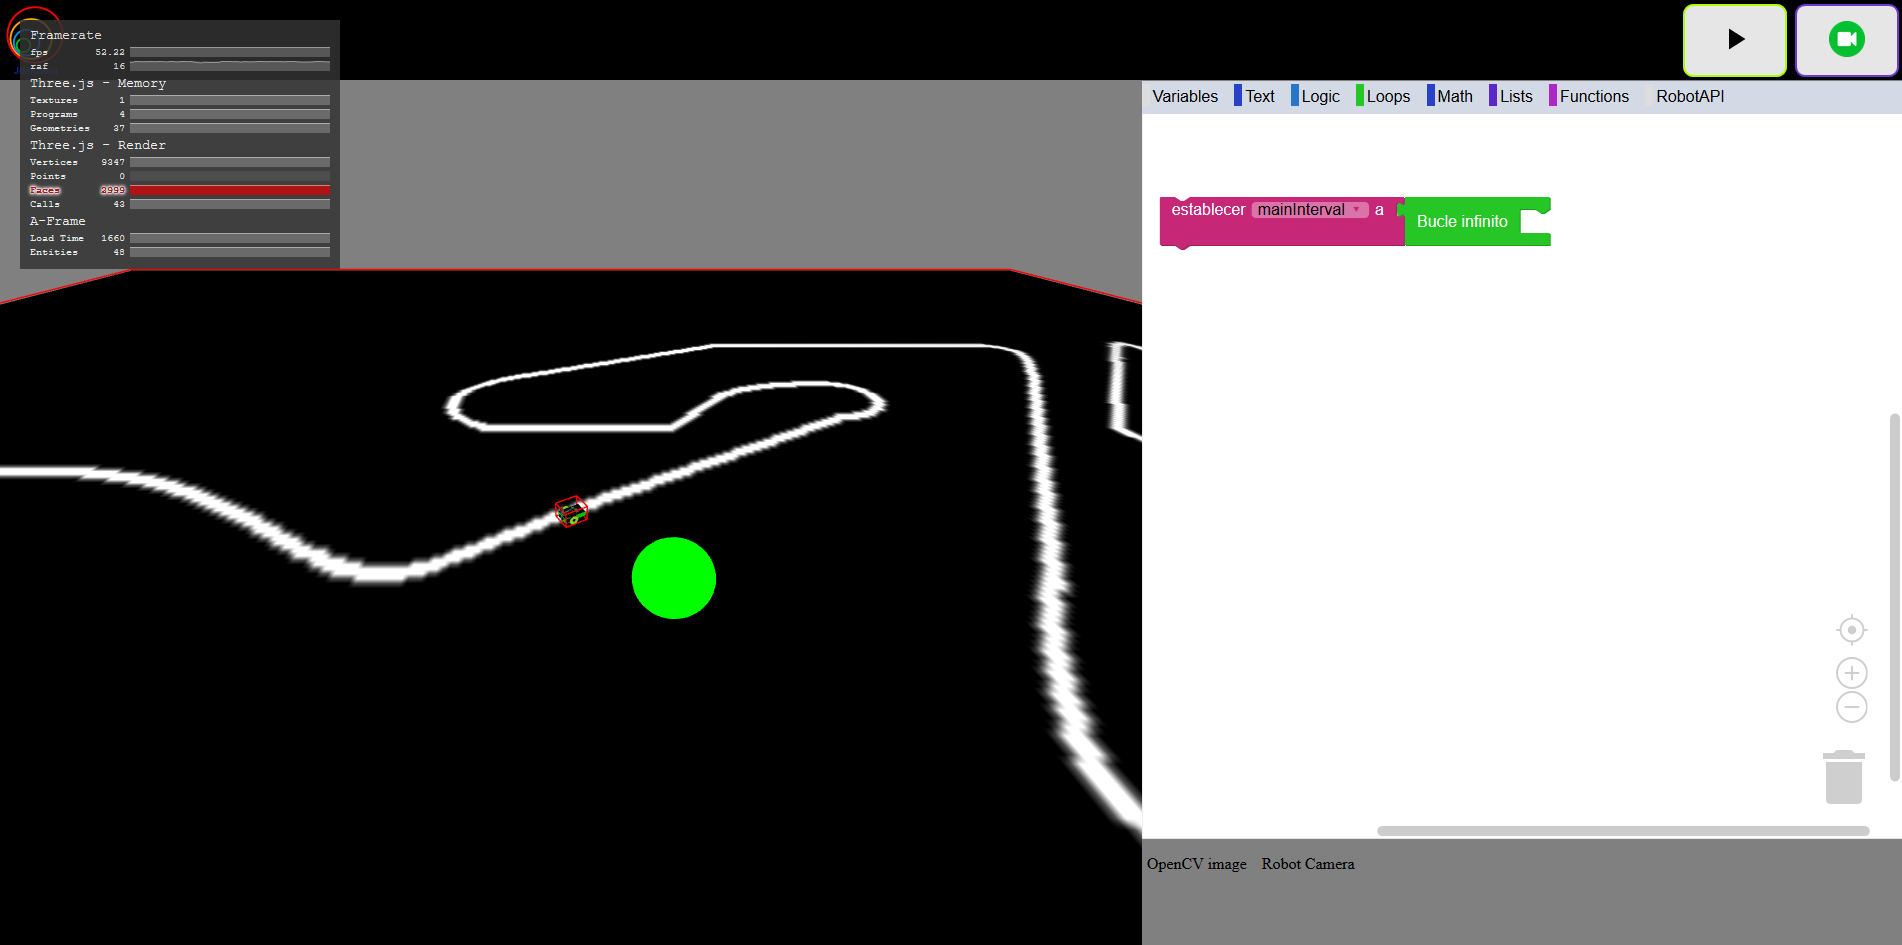
\includegraphics[width=1\textwidth]{img/interfaz-websim.png}
    \caption{Interfaz gráfica de \textit{WebSim}} \label{fig:websim}
\end{figure}

\subsection{Robot en WebSim}
\label{subsec:robot}
Para tener una entidad en \textit{A-Frame} que pueda ser programada por el usuario existe una clase en \textit{JavaScript} llamada \textit{RobotI}.
El constructor de esta clase es un método obligatorio y es al primero que se llama cuando se instancia un objeto. 
Tiene un parámetro de entrada que es una cadena de caracteres con el identificador de la etiqueta \textit{HTML} en la que se encuentra el robot simulado. 
Además de inicializar el robot, la clase contiene una serie de variables para su configuración: 
\begin{itemize}
    \item \textit{\textbf{defaultDistanceDetection}}: declara la distancia máxima en la que los sensores de ultrasonido detectan un objeto.
    \item \textit{\textbf{defaultNumOfRays}}: declara el número de rayos que se simulan para detectar objetos. Abarca un ángulo de 180 grados y, por lo tanto, cuanto mayor sea el número, más precisión habrá en la detección de objetos. 
    \item \textit{\textbf{robot}}: crea la unión entre la clase y la entidad del robot simulado en \textit{A-Frame}.
    \item \textit{\textbf{initialPosition}}: en la inicialización del robot, obtiene del \textit{HTML} la posición del robot y la guarda en esta variable.  
    \item \textit{\textbf{initialRotation}}: en la inicialización del robot, obtiene del \textit{HTML} la rotación del robot y la guarda en esta variable.  
    \item \textit{\textbf{activeRays}}: es una variable de tipo \textit{boolean} y permite saber si los rayos del sensor de ultrasonidos están activos no.
    \item \textit{\textbf{distanceArray}}. Es un objeto en \textit{JavaScript} con tres variables tipo \textit{array} y almacena la distancia con los objetos detectada por los sensores de ultrasonido. Las variables están diferenciadas en derecha, centro e izquierda y permite conocer donde se encuentra la ubicación del objeto detectado. 
    \item \textit{\textbf{understandedColors}}: variable que permite asociar un color como tipo \textit{string} a sus valores de filtro en el espacio \textit{RGB}. Esto permite hacer más simple la detección de los objetos para los usuarios ya que con el nombre del color se puede realizar el filtro sin necesidad de tener conocimientos sobre visión artificial.
    \item \textit{\textbf{velocity}}: variable que guarda la velocidad del robot en los distintos ejes (x,y,z). En el eje X se almacena la velocidad en el plano horizontal y en el eje Z la velocidad de giro. La velocidad del eje Y será útil en el desarrollo del proyecto ya que es la que otorga velocidad de elevación. 
\end{itemize}

Además, el constructor llama a los métodos para inicializar los motores y sensores que tienen sus propios métodos para su manejo. \\

Para enviar al \textit{robot} el código programado por el usuario se hace uso del módulo \textit{brains} en \textit{JavaScript}. En este se crea un ``hilo'' en el método \textit{runBrain} que guarda el código escrito en el editor en un \textit{array} y lo ejecuta periódicamente gracias a la función \textit{timeOut} de \textit{JavaScript}.

Este módulo también dispone de un método para parar el ``cerebro'' y reanudarlo después con un código distinto.
\begin{lstlisting}[language=javascript, caption=Método \textit{runBrain} para ejecutar el código del usuario]
brains.runBrain = (robotID, code) =>{
  code = 'async function myAlgorithm(){\n'+code+'\n}\nmyAlgorithm();';
  brains.threadsBrains.push({
    "id": robotID,
    "running": true,
    "iteration": brains.createTimeoutBrain(code, Websim.robots.getHalAPI(robotID), robotID),
    "codeRunning": code
  });
}
\end{lstlisting}

\begin{lstlisting}[language=javascript, caption=Métodos \textit{resumeBrain} y \textit{stopBrain} para parar/reanudar el cerebro del robot]
brains.resumeBrain = (robotID, code) =>{
  code = 'async function myAlgorithm(){\n'+code+'\n}\nmyAlgorithm();';
  var threadBrain = brains.threadsBrains.find((threadBrain)=> threadBrain.id == robotID);
  threadBrain.iteration = brains.createTimeoutBrain(code, Websim.robots.getHalAPI(robotID), robotID);
  threadBrain.running = true;
  threadBrain.codeRunning = code;
}
brains.stopBrain = (robotID) =>{
  var threadBrain = brains.threadsBrains.find((threadBrain)=> threadBrain.id == robotID);
  stopTimeoutRequested = true;
  clearTimeout(threadBrain.iteration);
  threadBrain.running = false;
}
\end{lstlisting}

%%modulo brains

% Para su implementación se ha creado el módulo \textit{brains} en \textit{JavaScript}, que contiene el método \textit{runBrains}, que ejecuta un ``hilo'' para cada \textit{robot} existente en la escena. Además contiene los métodos \textit{stopBrain} y \textit{resumeBrain} que paran y reanudan el cerebro del robot correspondiente.

\subsection{Drivers de sensores}
\label{subsec:driversSensores}
El robot consta de sensores simulados con \textit{A-Frame}. Los drivers permiten que el usuario, vía \textit{JavaScript}, pueda acceder a estos y obtener su información. En este entorno disponemos de los siguientes sensores: 

\begin{itemize}
    \item \textbf{Ultrasonido}: permite detectar obstáculos en un radio de 180 grados en la parte frontal del robot. En \textit{A-Frame} se simula gracias al atributo \textit{raycaster} el cual permite conocer el punto de intersección entre un rayo emitido y un objeto. Para la simulación de este sensor se usan los componentes \textit{followBody} (para anclar un \textit{raycaster} al robot y que pueda seguir la posición del robot) e \textit{intersectionHandler} (que crea un manejador para controlar el evento que lanza un \textit{raycaster} cuando un objeto se interpone en el rayo que emite). Además, este componente es capaz de detectar el identificador del \textit{raycaster} y la distancia a la que es detectado.
    
    \item \textbf{Cámara}: obtiene una imagen con lo que capta el robot de la escena. Para su simulación se ha creado el atributo \textit{spectator} y permite mostrar la visión del robot en primera persona. 
    
    \item \textbf{Infrarrojos}: dispositivo que está compuesto de un LED infrarrojo y un fototransistor siendo capaz de detectar si el objeto con el que choca la luz emitida por el LED es una superficie blanca (la luz rebota y llega hasta el fotoreceptor) o negra (la superficie absorbe toda la luz y no llega al fotoreceptor). 
    Para simular este sensor se emplea una cámara y se recorta la imagen obtenida para quedarse con los píxeles de la parte inferior (con una dimensión de 5x150px). La función del \textit{HAL API} que hace referencia a este sensor es \textit{readIR(color)} siendo el parámetro pasado a la función un color en formato de \textit{string} que toma como variable \textit{undestandedColors} para obtener los valores del filtro correspondiente. De tal manera, después del filtrado se obtiene una imagen según la posición en la que se encuentre la línea a seguir y según donde esté el centro devuelve distintos valores: \textit{0} si la línea se encuentra entre los píxeles 57 y 93 de la imagen, \textit{1} entre los píxeles 0 y 57, \textit{2} si la línea está entre 93 y 150 y \textit{3} si no detecta la línea.
    
    \item \textbf{Odómetro}: obtiene la posición absoluta del robot durante la ejecución del código. Para la simulación de los sensores de odometría se ha hecho uso del sistema de coordenadas y rotación de \textit{A-Frame} y se ha hecho el cálculo a través de su \textit{API} en \textit{JavaScript}. 
\end{itemize}
\clearpage
En la tabla \ref{tab:tablaSensores} se explican todas las funciones del \textit{HAL API} que hacen referencia a los sensores. 

\begin{table}[H]
\caption{Métodos (HAL API) de los sensores del robot.}
\vspace{0.5cm}
\label{tab:tablaSensores}
\resizebox{\textwidth}{!}{%
\begin{tabular}{|c|c|c|ll}
\cline{1-3}
\textbf{Método} & \textbf{Descripción} & \textbf{Salida} &  &  \\ \cline{1-3}
.getDistance() & \begin{tabular}[c]{@{}c@{}}Devuelve la distancia entre el robot\\  y la intersección del raycaster en el centro\end{tabular} & number(metros) &  &  \\ \cline{1-3}
.getDistances() & \begin{tabular}[c]{@{}c@{}}Devuelve la distancia entre el robot y\\ la intersección con cada una de los raycaster\end{tabular} & list number(metros) &  &   \\ \cline{1-3}
.readIR(color) & \begin{tabular}[c]{@{}c@{}}Recorta la imagen, filtra y calcula el centro\\ del objeto con el color pasado como argumento\end{tabular} & number &  &  \\ \cline{1-3}
.getRotation() & \begin{tabular}[c]{@{}c@{}}Retorna un objeto con la orientación \\ del robot en los 3 ejes\end{tabular} & \begin{tabular}[c]{@{}c@{}}\{x:number,\\ y:number,\\ z:number\}\end{tabular} &  &  \\ \cline{1-3}
.getPosition() & Obtiene la posición del robot en la escena & \begin{tabular}[c]{@{}c@{}}\{x:number,\\ y:number,\\ z:number\}\end{tabular} &  &  \\ \cline{1-3}
.getImage() & Devuelve la imagen de la cámara del robot & cv.Mat() &  &  \\ \cline{1-3}
.getObjectColor(color) & \begin{tabular}[c]{@{}c@{}}Devuelve un objeto con la posición del elemento\\ detectado por la cámara del color pasado por parámetro\end{tabular} & \begin{tabular}[c]{@{}c@{}}\{center:{[}x.y{]},\\ area: int\}\end{tabular} &  &  \\ \cline{1-3}
.getObjectColorRGB(valorBajo,valorAlto) & \begin{tabular}[c]{@{}c@{}}Devuelve un objeto con la posición del elemento\\ detectado por la cámara con los valores pasados por parámetro\end{tabular} & \begin{tabular}[c]{@{}c@{}}\{center:{[}x.y{]},\\ area: int\}\end{tabular} &  &  \\ \cline{1-3}
\end{tabular}%
}
\end{table}

\subsection{Drivers de actuadores}
\label{subsec:driversMotores}

La función de los actuadores es otorgar movimiento al cuerpo del robot simulado en \textit{A-Frame}. Con los métodos creados, además, no es necesario mandarle órdenes constantemente, si no que es suficiente con mandar la instrucción una vez y el robot seguirá ejecutándola hasta que reciba una nueva.  

Para que el robot siga las órdenes mandadas existen los siguientes métodos: 
\begin{itemize}
    \item \textit{\textbf{getV}}: Método para conocer la velocidad lineal ordenada al robot.
    \item \textit{\textbf{getW}}: Método que devuelve la velocidad angular comandada.
    \item \textit{\textbf{setV}}: Método que permite ordenar velocidad lineal al robot.
    \item \textit{\textbf{setL}}: Método para que el usuario comande la velocidad angular del robot. 
    \item \textit{\textbf{move}}: Método que sirve para ordenar tanto velocidad lineal como angular. 
\end{itemize}
Después de llamar a cada uno de estos métodos, se guarda la velocidad pasada por parámetro en la variable interna llamada \textit{velocity} y, para calcular la posición en el escenario simulado con \textit{A-Frame} es necesaria la siguiente función:

\begin{lstlisting}[language=javascript, caption=Función para actualizar la posición del robot en el escenario]
updatePosition(rotation, velocity, robotPos){
  let x = velocity.x/10 * Math.cos(rotation.y * Math.PI/180);
  let z = velocity.x/10 * Math.sin(-rotation.y * Math.PI/180);
  robotPos.x += x;
  robotPos.z += z;
  return robotPos;
}
\end{lstlisting}

En esta función se establece la nueva posición relativa para el objeto. En cada iteracción se calcula y se establece nueva posición y rotación del robot. Además, gracias a la función de \textit{JavaScript} llamada \textit{setTimeout},
se establece un temporizador para actualizar la posición del robot llamando a la función \textit{updatePosition} iterativamente cada cierto periodo de tiempo. Esto permite simplificar el código ya que hace que no es necesario mandar órdenes al robot constantemente. 

En la tabla \ref{tab:tablaMotores} se explican todas las funciones del \textit{HAL API} que hacen referencia a los actuadores.

\begin{table}[H]
  \begin{center}
    \caption{Métodos (HAL API) de los actuadores del robot.}
    \vspace{0.5cm}
    \label{tab:tablaMotores}
    \begin{tabular}{|c|c|} 
    \hline
      \textbf{Método} & \textbf{Descripción}\\
      \hline
.setV(integer) & \begin{tabular}[c]{@{}c@{}}Mueve hacia delante o atrás el robot.\\\end{tabular} \\ \hline
.setW(integer) & \begin{tabular}[c]{@{}c@{}}Hace girar al robot.\\\end{tabular} \\ \hline
.move(integer, integer) & \begin{tabular}[c]{@{}c@{}}Mueve el robot hacia delante/atrás y gira al mismo tiempo.\\ \end{tabular} \\ \hline
.getV() & \begin{tabular}[c]{@{}c@{}}Obtener la velocidad lineal configurada en el robot.\\ \end{tabular} \\ \hline
.getW() & \begin{tabular}[c]{@{}c@{}}Obtener la velocidad angular configurada en el robot.\\ \end{tabular} \\ \hline
    \end{tabular}
  \end{center}
\end{table}
